\chapter{ВЫВОД НЕОБХОДИМЫХ УРАВНЕНИЙ}
    \section{Конфигурации модели}
        Для написания алгоритма сканирования в первую очередь необходимо составить математическую модель сканера, то есть вывести соответствующие уравнения, по которым будут рассчитываться координаты точек в сцене. При этом возможно несколько вариантов для вывода необходимых уравнений.

        \subsection{Модель в системе координат принтера}
            Первая модель подразумевает расчёт в системе координат принтера, привязана к реальным элементам в сборке и отражает реальную конструкцию модуля. Главными параметрами являются $ H $ --- высота камеры над столом и $ \alpha $ --- угол наклона камеры от вертикали. В данном варианте предполагается, что стол -- рабочая поверхность -- находится в плоскости $ XY $, лазер излучает перпендикулярно столу и камера имеет поворот только вокруг оси $ Y $. При этом считается, что лазер не имеет поворота вокруг своей оси \hl{ХЗ КАК ПО ДРУГОМУ ЩАС НАПИСАТЬ}.

            \begin{figure}[!ht]\label{pic:first_model}
                \centering
                \includegraphics[width=0.75\linewidth]{first_model}
                \caption{Чертёж поясняющий вычисления}
            \end{figure}
            Таким образом приходим к следующим уравнениям
            \begin{equation}\label{eq:first_model}
                \begin{aligned}
                    z &= H\dfrac{\sin\left(\beta-\beta_0\right)}{\sin\left(\left(\beta-\beta_0\right)-\alpha\right)\cos\left(\alpha+\beta_0\right)}\\
                    x &= x_\text{к} - H\tg\left(\alpha+\beta_0\right)\\
                    y &= y_\text{к} - \left(H-z\right)\dfrac{\Delta u}{f\cos\alpha}\\
                \end{aligned}
            \end{equation}

            Преимущества этой модели:
            \begin{itemize}
                \item $ H $ можно измерять напрямую
                \item рассчитанные значения координат сразу в системе координат принтера
                \item отражает реальную конструкцию сканера
                \item координата $ x $ константа относительно камеры
            \end{itemize}
            
            Недостатки:
            \begin{itemize}
                \item много тригонометрических преобразований
                \item при изменении высоты камеры необходимы новые замеры
                \item большое количество допущений, как следствие много возможностей для ошибок
            \end{itemize}

        \subsection{Модель в системе координат камеры}
            Вторая модель основывается на теоретических величинах и расчёт происходит в два этапа. Первый -- расчёт координат относительно камеры, второй -- преобразование в систему координат принтера. В этом методе главными параметрами являются высота камеры $ H $ над рабочей плоскостью и угол между камерой и лазером $ \alpha $, но они рассчитываются теоретически и не совпадают с аналогичными из предыдущего метода. В этой модели считается, что лазер не имеет поворота вокруг своей оси, все остальные компоненты могут располагаться произвольно.
            
            Для преобразования между двумя системами координат необходимо знать матрицу поворота системы камеры относительно системы принтера. С помощью пакета opencv можно полностью определить положение камеры в пространстве используя шахматный паттерн.
            \begin{figure}[!ht]\label{pic:second_model}
                \centering
                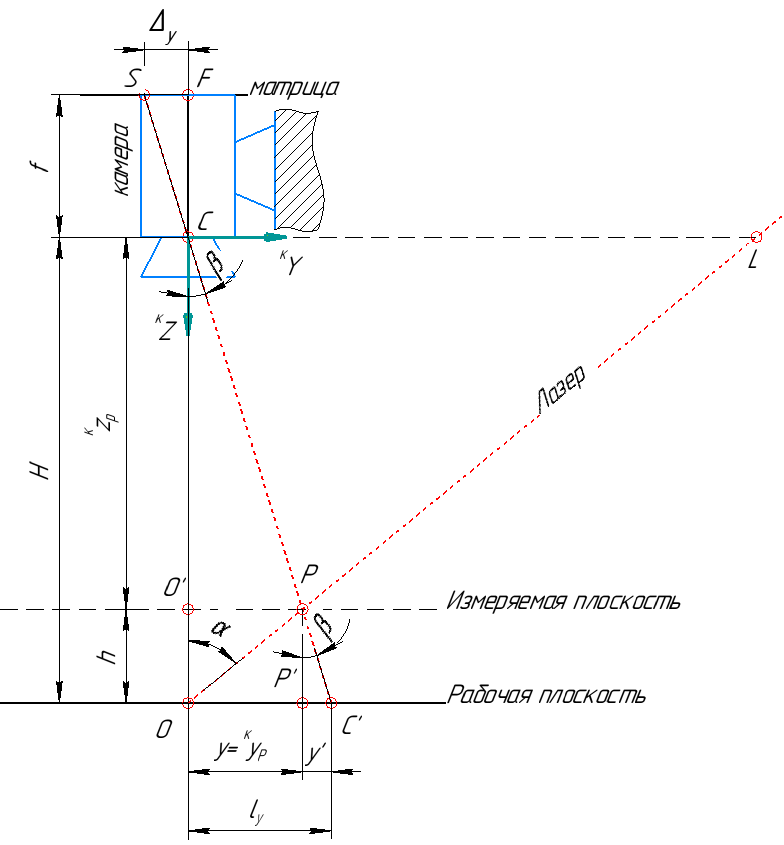
\includegraphics[width=0.75\linewidth]{second_model}
                \caption{Чертёж поясняющий вычисления}
            \end{figure}
            В системе координат камеры получаем:
            \begin{equation}\label{eq:second_model}
                \begin{aligned}
                    \prescript{\text{к}}{}{x}_p = H\frac{\tg\alpha\frac{\Delta x}{f}}{\tg\alpha+\frac{\Delta y}{f}}\\
                    \prescript{\text{к}}{}{y}_p = H\frac{\tg\alpha\frac{\Delta y}{f}}{\tg\alpha+\frac{\Delta y}{f}}\\
                    \prescript{\text{к}}{}{z}_p = H\frac{\tg\alpha}{\tg\alpha+\frac{\Delta v}{f}}
                \end{aligned}
            \end{equation}
            Для перевода в систему координат принтера:
            \begin{equation}
                \label{eq:coord_world}
                \begin{pmatrix}
                    x\\y\\z
                \end{pmatrix}
                =
                R
                \begin{pmatrix}
                    \prescript{\text{к}}{}{x}_p\\
                    \prescript{\text{к}}{}{y}_p\\
                    \prescript{\text{к}}{}{z}_p
                \end{pmatrix}
                +
                \begin{pmatrix}
                    x_\text{к}\\y_\text{к}\\z_\text{к}
                \end{pmatrix}
            \end{equation}
            Преимущества модели:
            \begin{itemize}
                \item отсутствие тригонометрии в расчётах координат
                \item параметры $ H $ и $ \alpha $ фиксированы
                \item меньшее количество допущений
            \end{itemize}
            \begin{itemize}
                \item сложно прямо измерить $ H $ и $ \alpha $, необходим теоретический расчёт
                \item необходима матрица поворота камеры
            \end{itemize}
        \subsection{Выбор модели}

    \section{Оценка теоретической погрешности}\label{sec:error}
    
    \section{Калибровка сканера}